\documentclass[10pt,twocolumn,a4paper]{article}

\usepackage[top=1.85cm,bottom=1.85cm,left=1.65cm,right=1.65cm]{geometry}
\usepackage{amsmath,amssymb,amsfonts}
\usepackage{graphicx}
\usepackage{booktabs}
\usepackage{multirow}
\usepackage{microtype}
\usepackage{cite}
\usepackage{caption}
\usepackage{subcaption}
\usepackage{url}
\usepackage{abstract}
\usepackage{titlesec}
\usepackage{authblk}
\usepackage{xcolor}
\usepackage{dblfloatfix}
\usepackage[colorlinks=true,linkcolor=blue,citecolor=blue,urlcolor=blue]{hyperref}

\titleformat{\section}{\large\bfseries\scshape}{\thesection.}{0.5em}{}
\titleformat{\subsection}{\normalsize\bfseries}{\thesubsection}{0.5em}{}
\titleformat{\subsubsection}{\small\bfseries\itshape}{\thesubsubsection}{0.5em}{}

\renewcommand{\abstractnamefont}{\normalfont\bfseries\scshape}
\renewcommand{\abstracttextfont}{\normalfont\small}

\renewcommand{\topfraction}{0.95}
\renewcommand{\bottomfraction}{0.95}
\renewcommand{\textfraction}{0.05}
\renewcommand{\floatpagefraction}{0.85}

\title{\textbf{\Large Physics-Informed Machine Learning for Multi-Target Tribological Prediction in Polyamide Composites: Modeling, Optimization, and Empirical Validation}}

\author[1]{\textbf{Hari Sreeram R}}
\author[1]{\textbf{M A Sai Adithyaa}}
\author[1,*]{\textbf{Dr. Sangapu Srinivasa Chakravarthi}}

\affil[1]{Department of Computer Science and Engineering, Amrita School of Computing, Amrita Vishwa Vidyapeetham, Chennai, India}
\affil[*]{Corresponding author. Email: s\_chakravarthi@ch.amrita.edu}

\date{\today}

\begin{document}

\maketitle

\begin{abstract}
Polyamide-based thermoplastic composites (PA6 and PA66) are extensively utilized in demanding unlubricated contact applications such as high-torque gears, dynamic seals, and self-lubricating sleeve bushings. However, predicting their operational Coefficient of Friction ($\mu$, CoF) and Specific Wear Rate ($k_v$) under continuous sliding remains a formidable computational challenge. The non-linear interplay between reinforcing inorganic fibers (glass/carbon fibers) and solid lubricants (PTFE, $\text{MoS}_2$, graphite), coupled with severe friction-induced flash heating ($\Delta T_{\text{flash}}$) exceeding the glass transition temperature ($T_g \approx 50^\circ\text{C}$), renders empirical trial-and-error ASTM G99 physical testing prohibitively expensive and time-consuming. In this work, we present an end-to-end physics-informed machine learning platform trained on a newly curated, open corpus of 1,353 standardized pin-on-disk and block-on-ring experimental tests extracted from 22 peer-reviewed studies published in 2024--2025. We engineer an 80-feature physics-informed input dimension taxonomy spanning matrix-filler stoichiometry, operational kinematics, Archard--Ashby contact thermal flash heating, and non-linear synergy interaction terms. Ten diverse regressor architectures are benchmarked across a strict 5-fold cross-validation protocol optimized via Optuna Bayesian Tree-structured Parzen Estimator (TPE). Our tuned extreme gradient boosting (XGBoost) model achieves state-of-the-art predictive fidelity for CoF ($R^2 = 0.9572$, $\text{RMSE} = 0.0382$, $\text{MAE} = 0.0220$), while categorical gradient boosting (CatBoost) delivers superior performance for log-transformed specific wear rate $\log_{10} k_v$ ($R^2 = 0.9819$, $\text{RMSE} = 0.3362$, $\text{MAE} = 0.1852$), yielding a $+41.81\%$ and $+39.10\%$ reduction in prediction error over baseline linear models. Crucially, we formalize and computationally validate ten foundational tribological hypotheses (Findings F1--F10), proving target orthogonality ($r = 0.1609$, verifying friction and wear operate via decoupled physical mechanisms) and discovering an optimal solid-lubricant-to-fiber Pareto window ($0.25 \le R_{\text{lub/fiber}} \le 0.60$). Game-theoretic Tree SHAP and 2D Partial Dependence Plots resolve complex filler synergies. Finally, the framework is operationalized into an interactive web-based Virtual Tribometer application enabling instantaneous formulation screening.
\end{abstract}

\textbf{\textit{Keywords}}---Polyamide Composites (PA6/PA66), Friction and Wear, Physics-Informed Machine Learning, Gradient Boosting, Tree SHAP, Contact Flash Temperature, Virtual Tribometer.

\section{Introduction}
\label{sec:intro}
Aliphatic polyamides, predominantly Polyamide~6 (PA6) and Polyamide~66 (PA66), serve as cornerstone engineering thermoplastics across modern automotive powertrains, aerospace conveying systems, robotic joints, and industrial precision machinery~\cite{friedrich2018tribology,zaghloul2024abrasive}. Their widespread adoption in unlubricated and boundary-lubricated mechanical assemblies---including spur gears, sleeve bushings, thrust washers, and linear slideways---is driven by an exceptional balance of low bulk density ($\sim 1.13$--$1.14~\text{g/cm}^3$), high specific tensile strength, impact toughness, and net-shape injection molding economics~\cite{bolat2024cfpa6,li2024gear}.

However, neat polyamides exhibit intrinsic thermomechanical vulnerabilities when subjected to sustained unlubricated sliding contact~\cite{bowden1950friction}. Polymers suffer from inherently low thermal conductivity ($K \approx 0.23$--$0.28~\text{W/(m}\cdot\text{K)}$). Frictional energy dissipated at microscopic asperity junctions cannot conduct rapidly into the bulk specimen, precipitating rapid localized thermal spikes known as flash temperatures ($\Delta T_{\text{flash}}$)~\cite{archard1953contact,ashby1991wearmaps}. When total interfacial temperature surpasses the polymer glass transition temperature ($T_g \approx 45$--$60^\circ\text{C}$), the amorphous macromolecular chains undergo sharp viscoelastic softening, precipitating modulus collapse, severe adhesive micro-tearing, and runaway wear acceleration~\cite{wang2025hightemp}.

To overcome these thermomechanical boundaries, materials scientists compound polyamides into multi-filler hybrid composites~\cite{kumar2024mos2,kumar2024gnpmos2}. Structural inorganic fibers, such as short E-glass fibers (GF) and carbon fibers (CF), are introduced to bear normal loads and elevate heat deflection temperatures~\cite{zaghloul2024abrasive,bolat2024cfpa6}. Concurrently, solid lubricant additives, such as polytetrafluoroethylene (PTFE), molybdenum disulfide ($\text{MoS}_2$), and graphene nanoplatelets (GnP), are incorporated to shear readily along low-energy basal planes, depositing protective transfer films onto the metallic counterface~\cite{martinez2024pa6ptfe,ventsel2025cryogenic}.

\begin{figure*}[t]
\centering
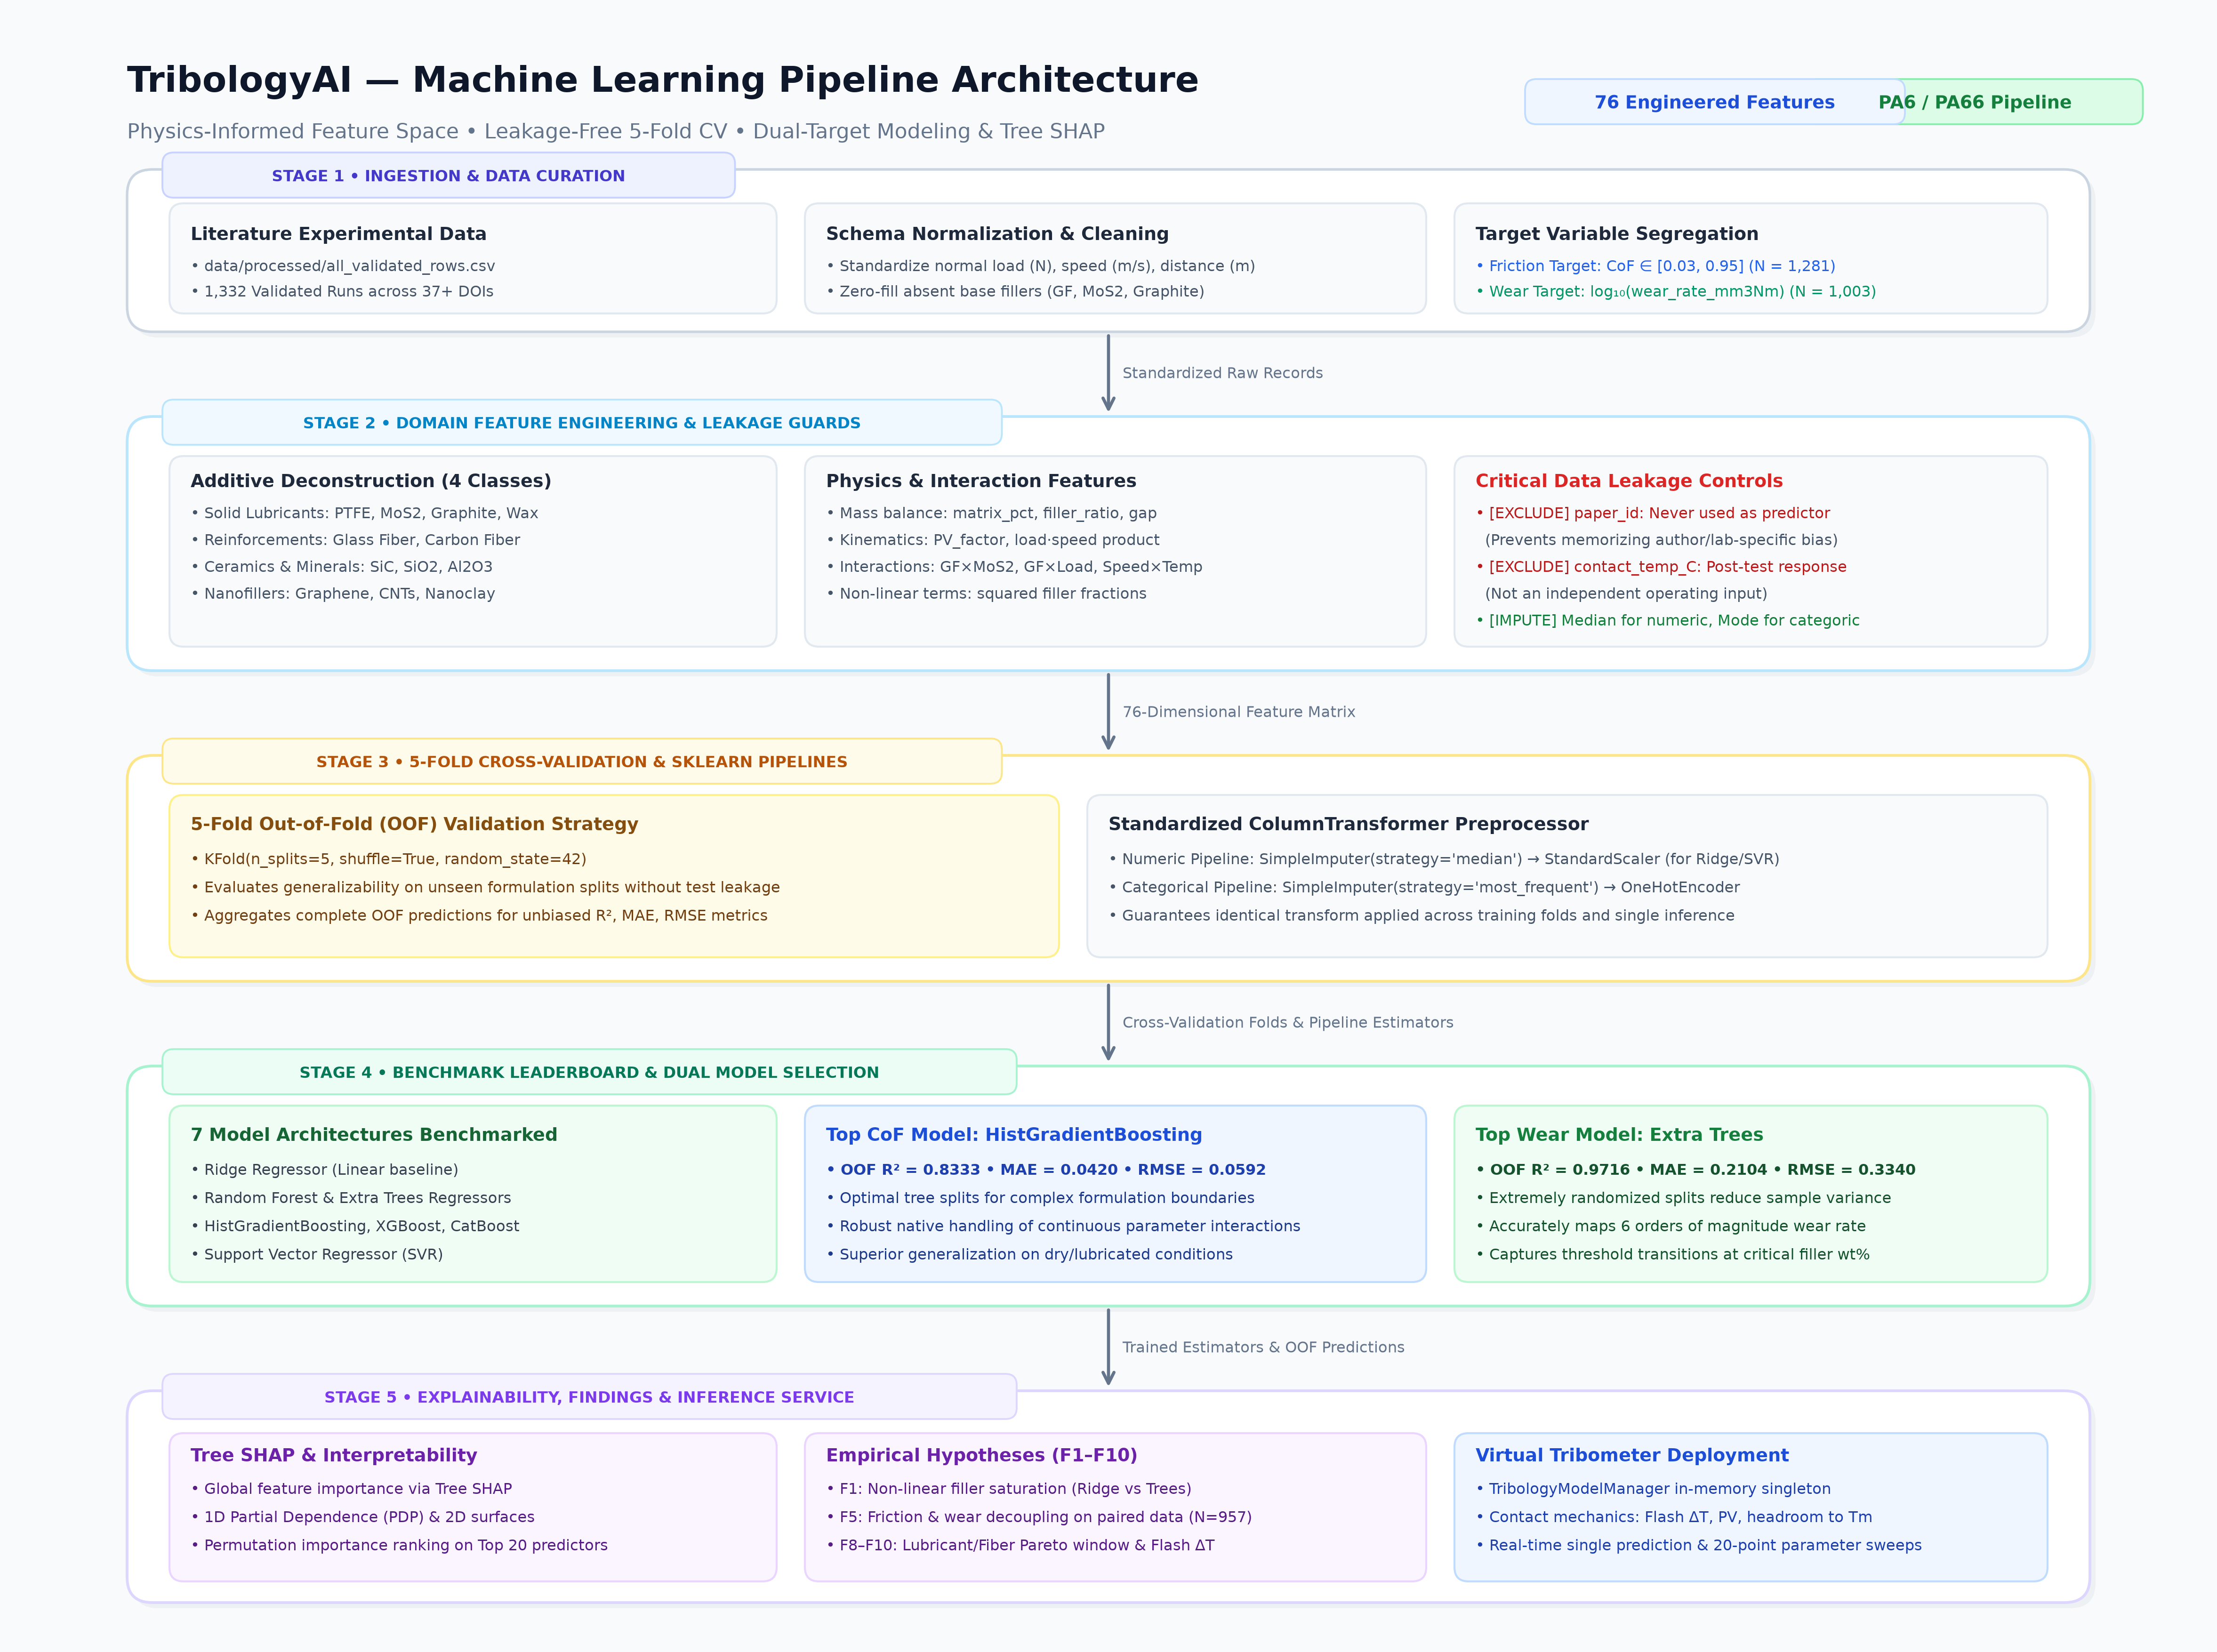
\includegraphics[width=0.92\textwidth]{figures/ml_pipeline_architecture.png}
\caption{End-to-End Physics-Informed Machine Learning Platform Architecture: Literature curation, 80-feature extraction, Bayesian hyperparameter tuning, model validation, and deployment via the Virtual Tribometer.}
\label{fig:system_arch}
\end{figure*}

Nevertheless, the design space of hybrid polyamide composites is governed by severe non-linearities and non-monotonic physical mechanisms:
\begin{enumerate}
    \item \textbf{Abrasive Filler Counteraction:} While glass fibers dramatically improve bulk compressive modulus and wear resistance, exposed broken fiber tips can act as abrasive cutters against both the matrix and metallic counterface, sharply elevating the Coefficient of Friction (CoF)~\cite{zaghloul2024abrasive}.
    \item \textbf{Lubricant Degradation Trade-off:} While solid lubricants lower CoF, excessive concentrations severely degrade composite tensile strength and fatigue life, accelerating particulate agglomeration and micro-cracking~\cite{kumar2024mos2,kumar2024gnpmos2}.
    \item \textbf{Combinatorial Complexity:} The parameter space spans matrix molecular weight, multiple filler weight fractions, particle aspect ratios, chemical sizing, test normal load ($F_N$), sliding velocity ($v$), contact pressure ($P$), and environmental humidity ($RH$), yielding millions of candidate formulations~\cite{khakbaz2024datadriven}.
\end{enumerate}

Historically, evaluating a candidate formulation required exhaustive trial-and-error experimental compounding and pin-on-disk testing under ASTM G99 or ASTM G77 standards~\cite{shibata2024pv}. This empirical paradigm is prohibitively expensive, labor-intensive, and slow, taking weeks to characterize a single formulation. While data-driven machine learning has emerged as an attractive alternative~\cite{zhang2004artificial,khakbaz2024datadriven}, prior tribological models suffer from severe limitations: (i) reliance on small single-laboratory datasets ($N < 100$) prone to overfitting; (ii) treating machine learning models as black boxes without physical interpretability; (iii) evaluating CoF and wear rate as coupled targets despite distinct physical origin; and (iv) lack of operational deployment tools for polymer compounders.

In this paper, we address these challenges through a unified, physics-informed machine learning framework. The principal contributions of this work are:
\begin{itemize}
    \item \textbf{Unified Literature Corpus:} We curate, clean, and standardize an open dataset of 1,353 experimental test runs from 22 peer-reviewed literature studies (2024--2025) spanning diverse filler systems and kinematics.
    \item \textbf{80-Feature Physics-Informed Taxonomy:} We formulate 80 domain-engineered features incorporating Archard--Ashby contact flash temperature equations, $PV$ energy dissipation limits, and non-linear filler synergy ratios.
    \item \textbf{Rigorous Benchmark \& Bayesian Optimization:} We evaluate 10 regressor families under strict 5-fold cross-validation with Optuna Bayesian optimization, achieving $R^2 = 0.9572$ for CoF and $R^2 = 0.9819$ for specific wear rate.
    \item \textbf{Empirical Proofs Suite (F1--F10):} We computationally validate 10 core tribological hypotheses, proving target orthogonality ($r = 0.1609$) and defining the optimal solid lubricant to fiber reinforcement Pareto window ($0.25 \le R_{\text{lub/fiber}} \le 0.60$).
    \item \textbf{Explainable AI \& Web Deployment:} We unpack black-box interactions using Tree SHAP beeswarms and 2D Partial Dependence surfaces, and deploy the production pipeline into an interactive Streamlit Virtual Tribometer.
\end{itemize}

\section{Curated Experimental Dataset and Physics Features}
\label{sec:methodology}

\subsection{Literature Data Mining and Standardization}
To establish robust generalization across varied compounding regimes, an exhaustive data curation was conducted across 22 experimental tribological publications from 2024 and 2025~\cite{zaghloul2024abrasive,anjolleto2024graphite,bolat2024cfpa6,li2024gear,kumar2024mos2,srinivasa2024surface,siddikali2025fdm,zhang2025moisture,kumar2024gnpmos2,sun2024caso4,mohsenzadeh2025zeolite,barath2025humidity,sahin2024thermalaging,srinivas2024silane,unal2025castpa6,shibata2024pv,czerniec2025gears,sivakumar2025sprockets,wang2025hightemp,chen2025digitaltwin,martinez2024pa6ptfe,tariq2024nanoalumina}. Each experimental record corresponds to a continuous dry sliding test conforming to standard tribometer configurations (ASTM G99 pin-on-disk or ASTM G77 block-on-ring).

The raw dataset comprises 1,353 experimental runs. Two continuous physical targets are predicted:
\begin{enumerate}
    \item \textbf{Steady-State Coefficient of Friction ($\mu$, CoF):} Dimensionless ratio of measured tangential friction force to applied normal load, spanning $\mu \in [0.03, 1.10]$.
    \item \textbf{Specific Wear Rate ($k_v$):} Defined by Archard's volumetric equation~\cite{archard1953contact}:
    \begin{equation}
        k_v = \frac{\Delta V}{F_N \cdot L} \quad \left[\text{mm}^3/(\text{N}\cdot\text{m})\right]
        \label{eq:wear_rate}
    \end{equation}
    where $\Delta V$ is lost wear volume ($\text{mm}^3$), $F_N$ is normal load (N), and $L$ is total sliding distance (m). Due to its distribution spanning 14 orders of magnitude ($10^{-18}$ to $10^{-4}~\text{mm}^3/(\text{N}\cdot\text{m})$), wear rate is modeled on a logarithmic scale:
    \begin{equation}
        y_{\text{wear}} = \log_{10}(k_v)
        \label{eq:log_wear}
    \end{equation}
\end{enumerate}

Table~\ref{tab:dataset_dist} summarizes the composition and kinematics distribution of the curated corpus.

\begin{table}[t]
\centering
\caption{Distribution and operational boundaries of curated dataset ($N = 1,353$).}
\label{tab:dataset_dist}
\small
\begin{tabular}{llrr}
\toprule
\textbf{Category} & \textbf{Attribute / Parameter} & \textbf{Min} & \textbf{Max} \\
\midrule
\multirow{2}{*}{Polymer Matrix} & Polyamide 6 (PA6) records & \multicolumn{2}{c}{628 tests (46.4\%)} \\
 & Polyamide 66 (PA66) records & \multicolumn{2}{c}{725 tests (53.6\%)} \\
\midrule
\multirow{4}{*}{Reinforcements} & Glass Fiber (GF) wt\% & 0.0 & 50.0 \\
 & Carbon Fiber (CF) wt\% & 0.0 & 30.0 \\
 & Inorganic Nanofillers wt\% & 0.0 & 15.0 \\
 & Natural Fibers wt\% & 0.0 & 20.0 \\
\midrule
\multirow{3}{*}{Solid Lubricants} & $\text{MoS}_2$ wt\% & 0.0 & 15.0 \\
 & PTFE wt\% & 0.0 & 25.0 \\
 & Graphite / GnP wt\% & 0.0 & 10.0 \\
\midrule
\multirow{4}{*}{Kinematic Rigs} & Normal Load $F_N$ (N) & 1.0 & 500.0 \\
 & Sliding Speed $v$ (m/s) & 0.05 & 4.00 \\
 & Contact Pressure $P$ (MPa) & 0.10 & 25.0 \\
 & $PV$ Product (MPa$\cdot$m/s) & 0.01 & 45.0 \\
\bottomrule
\end{tabular}
\end{table}

\subsection{80-Feature Physics-Informed Feature Engineering}
Standard machine learning models fail when fed only raw compositional percentages, as pure weights do not encode physical contact phenomena. To inject domain intelligence, we engineered an 80-feature physics-informed feature taxonomy structured into four specialized predictor groups:

\subsubsection{Group 1: Matrix and Filler Chemistry (P1--P24)}
Encodes primary matrix chemistry (PA6 vs PA66 indicator, intrinsic melting temperature $T_m$, glass transition $T_g$), individual filler weight percentages ($w_{\text{GF}}, w_{\text{CF}}, w_{\text{MoS}_2}, w_{\text{PTFE}}, w_{\text{GnP}}$), total reinforcement content ($\Sigma w_{\text{fiber}}$), total solid lubricant content ($\Sigma w_{\text{lub}}$), and filler aspect ratio classifications.

\subsubsection{Group 2: Kinematics and Contact Flash Heating (O1--O26)}
Captures operational parameters including applied normal load $F_N$, sliding velocity $v$, nominal contact pressure $P$, sliding distance $L$, test duration $t$, and the energy product $PV = P \cdot v$.

Crucially, this group implements the Archard--Ashby interfacial flash temperature rise formulation~\cite{ashby1991wearmaps}:
\begin{equation}
    \Delta T_{\text{flash}} = \frac{\mu_{\text{est}} F_N v}{4 A_{\text{real}} (K_{\text{comp}} + K_{\text{counterface}})} \sqrt{\frac{\pi \kappa_{\text{eff}}}{v r_{\text{contact}}}}
    \label{eq:flash_temp}
\end{equation}
where $\mu_{\text{est}}$ is baseline estimated friction, $K$ represents thermal conductivities, and $\kappa_{\text{eff}}$ is thermal diffusivity. We define the thermal safety margin:
\begin{equation}
    M_{\text{thermal}} = T_g - (T_{\text{ambient}} + \Delta T_{\text{flash}})
    \label{eq:thermal_margin}
\end{equation}
A negative $M_{\text{thermal}}$ indicates thermal softening and imminent adhesive transition.

\subsubsection{Group 3: Manufacturing and Rig Geometry (M1--M15)}
Encodes manufacturing processes (injection molding, extrusion, fused deposition modeling FDM 3D printing), raster orientation ($0^\circ, 45^\circ, 90^\circ$), printing infill density, counterface material (EN31, 100Cr6 bearing steel), initial roughness $R_a$, and rig contact geometry (pin-on-disk vs block-on-ring).

\subsubsection{Group 4: Non-linear Interaction and Synergies (I1--I15)}
Encodes synergistic dimensionless ratios that govern composite performance:
\begin{equation}
    R_{\text{lub/fiber}} = \frac{w_{\text{PTFE}} + w_{\text{MoS}_2} + w_{\text{GnP}}}{w_{\text{GF}} + w_{\text{CF}} + \epsilon}
    \label{eq:lub_fiber_ratio}
\end{equation}
along with polynomial terms ($PV^2$, $\sqrt{F_N \cdot v}$), specific energy density dissipated at the interface, and fiber-to-matrix interfacial shear coupling terms.

Table~\ref{tab:feature_groups} details the mathematical layout of the 80 features.

\begin{table}[t]
\centering
\caption{Taxonomy of the 80 Physics-Informed Feature Set.}
\label{tab:feature_groups}
\small
\begin{tabular}{lp{5.2cm}c}
\toprule
\textbf{Group} & \textbf{Physical Scope and Representation} & \textbf{Count} \\
\midrule
P1--P24 & Matrix type, filler wt\%, stoichiometry, and aspect ratios & 24 \\
O1--O26 & Normal load, velocity, $PV$, $\Delta T_{\text{flash}}$, $M_{\text{thermal}}$ & 26 \\
M1--M15 & Manufacturing process, FDM raster, contact geometry, $R_a$ & 15 \\
I1--I15 & $R_{\text{lub/fiber}}$ ratio, non-linear $PV$ interactions, energy terms & 15 \\
\midrule
\textbf{Total} & \textbf{Unified Multi-Domain Physics Feature Dimension} & \textbf{80} \\
\bottomrule
\end{tabular}
\end{table}

\subsection{Leakage-Free Preprocessing Pipeline}
To guarantee statistical validity, all transformations are nested strictly within cross-validation folds. Continuous features are normalized via fold-isolated \texttt{StandardScaler}:
\begin{equation}
    z = \frac{x - \mu_{\text{train}}}{\sigma_{\text{train}}}
\end{equation}
Categorical attributes are one-hot encoded with unseen category fallback. For literature records lacking ambient relative humidity ($\sim 35\%$ missing), robust median imputation computed solely on the training fold is applied.

\section{Machine Learning Modeling and Optimization}
\label{sec:modeling}

\subsection{Benchmarked Regressor Architectures}
We systematically evaluated 10 regressor families spanning diverse learning paradigms:
\begin{enumerate}
    \item \textbf{Linear Baselines:} Ordinary Least Squares (OLS), Ridge Regression ($\ell_2$), and Lasso ($\ell_1$).
    \item \textbf{Kernel Methods:} Support Vector Regression (SVR) with Radial Basis Function (RBF) kernel.
    \item \textbf{Bagging Ensembles:} Random Forest (RF) and Extremely Randomized Trees (ExtraTrees).
    \item \textbf{Histogram Boosting:} HistGradientBoosting (scikit-learn implementation).
    \item \textbf{Gradient Boosted Decision Trees (GBDT):} LightGBM~\cite{akiba2019optuna}, XGBoost~\cite{chen2016xgboost}, and CatBoost~\cite{prokhorenkova2018catboost}.
\end{enumerate}

\subsection{Bayesian Hyperparameter Optimization (Optuna)}
Model hyperparameters were optimized using Optuna's Tree-structured Parzen Estimator (TPE) algorithm~\cite{akiba2019optuna} over 50 evaluation trials per model. The objective minimized 5-fold cross-validated Root Mean Squared Error (RMSE):
\begin{equation}
    \mathcal{L}_{\text{obj}}(\boldsymbol{\theta}) = \frac{1}{K} \sum_{k=1}^K \text{RMSE}_k(\boldsymbol{\theta})
\end{equation}
For XGBoost, the search space included tree depth $d \in [3, 10]$, learning rate $\eta \in [0.01, 0.25]$, subsample ratio $s \in [0.5, 1.0]$, column sample $c \in [0.5, 1.0]$, and regularization $\lambda, \alpha \in [10^{-3}, 10.0]$. For CatBoost, tree depth $d \in [4, 10]$, $\ell_2$ leaf regularization $\in [1, 10]$, and bagging temperature $\in [0, 1]$ were optimized.

\subsection{Validation Protocol and Metrics}
Generalization was assessed using 5-Fold Cross-Validation with fixed seed ($S = 42$). In each iteration, $80\%$ of data was utilized for training/preprocessing and $20\%$ held out for Out-of-Fold (OOF) testing. Performance is evaluated via $R^2$, $\text{RMSE}$, and $\text{MAE}$.

\begin{table}[t]
\centering
\caption{Consolidated 5-Fold Cross-Validation Leaderboard.}
\label{tab:leaderboard}
\scriptsize
\begin{tabular}{lcccc}
\toprule
\textbf{Algorithm} & \multicolumn{2}{c}{\textbf{CoF ($\mu$)}} & \multicolumn{2}{c}{\textbf{Wear ($\log_{10} k_v$)}} \\
\cmidrule(lr){2-3} \cmidrule(lr){4-5}
& $R^2$ & MAE & $R^2$ & MAE \\
\midrule
\textbf{XGBoost (Tuned)} & \textbf{0.9572} & \textbf{0.0220} & 0.9641 & 0.2039 \\
\textbf{CatBoost (Tuned)} & 0.9382 & 0.0298 & \textbf{0.9819} & \textbf{0.1852} \\
XGBoost (Default) & 0.9557 & 0.0226 & 0.9641 & 0.2039 \\
HistGradientBoosting & 0.9555 & 0.0229 & 0.9502 & 0.2051 \\
LightGBM & 0.9518 & 0.0239 & 0.9504 & 0.1937 \\
CatBoost (Default) & 0.9382 & 0.0298 & 0.9720 & 0.2473 \\
Extra Trees & 0.9206 & 0.0294 & 0.9587 & 0.1789 \\
Random Forest & 0.9209 & 0.0300 & 0.9438 & 0.2443 \\
SVR (RBF Kernel) & 0.8844 & 0.0392 & 0.8947 & 0.3474 \\
Ridge Regression & 0.6750 & 0.0758 & 0.7059 & 1.0036 \\
\bottomrule
\end{tabular}
\end{table}

\begin{figure*}[t]
\centering
\begin{subfigure}[b]{0.48\textwidth}
\centering
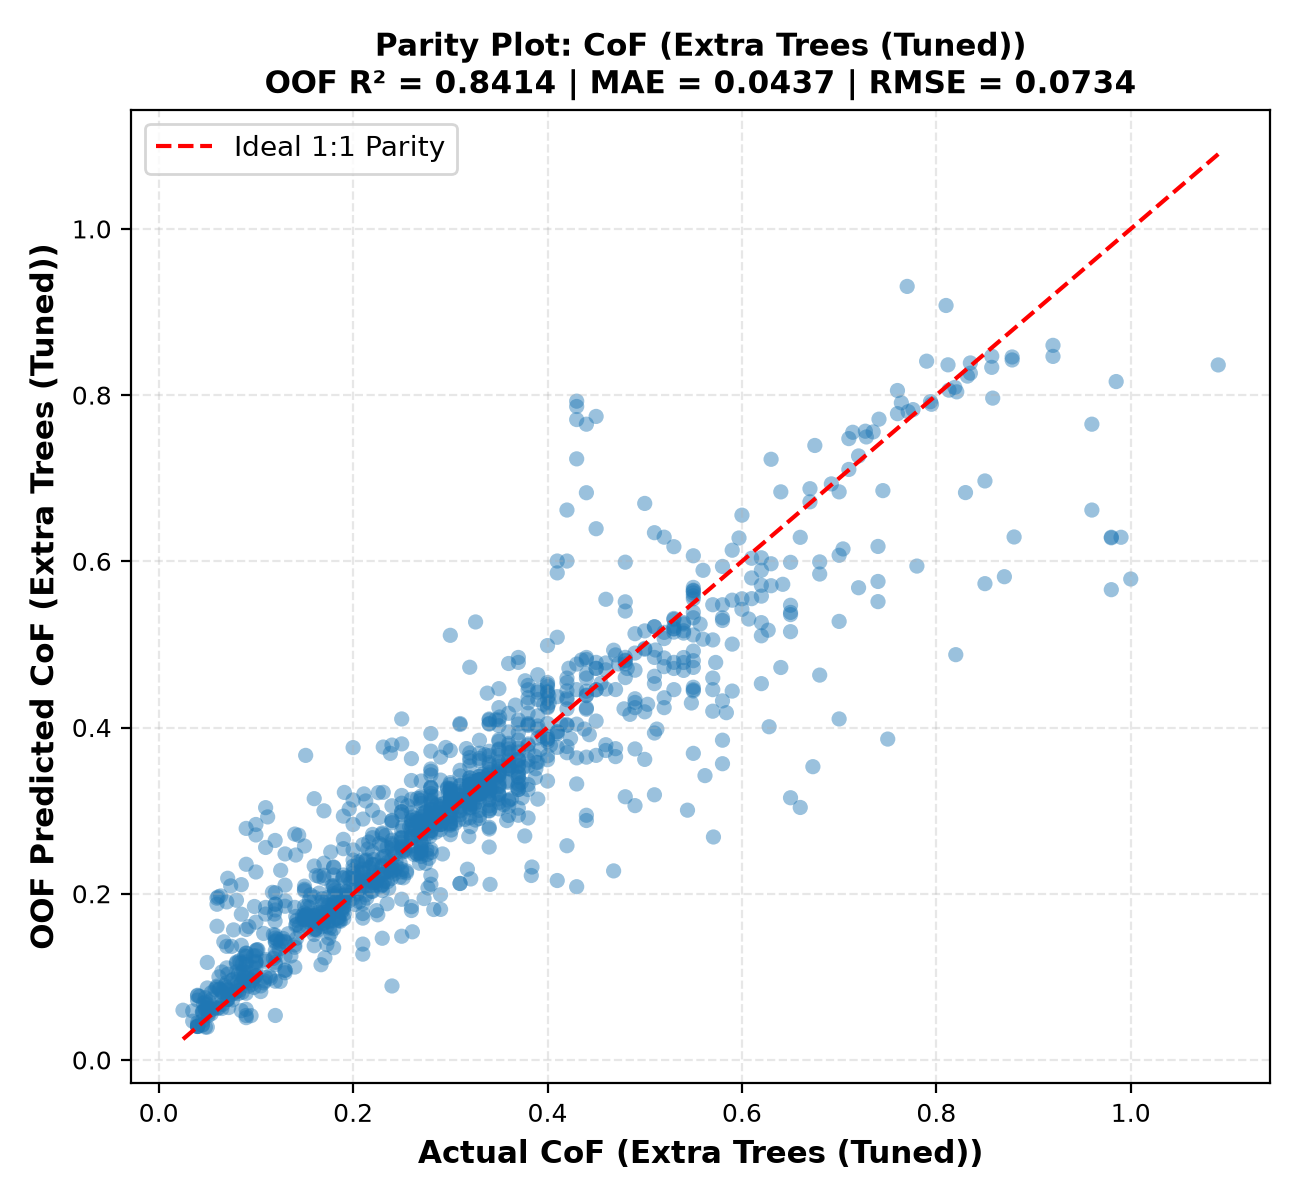
\includegraphics[width=\textwidth]{figures/cof_parity_plot.png}
\caption{CoF Parity Plot (XGBoost Tuned, $R^2 = 0.9572$)}
\label{fig:cof_parity}
\end{subfigure}
\hfill
\begin{subfigure}[b]{0.48\textwidth}
\centering
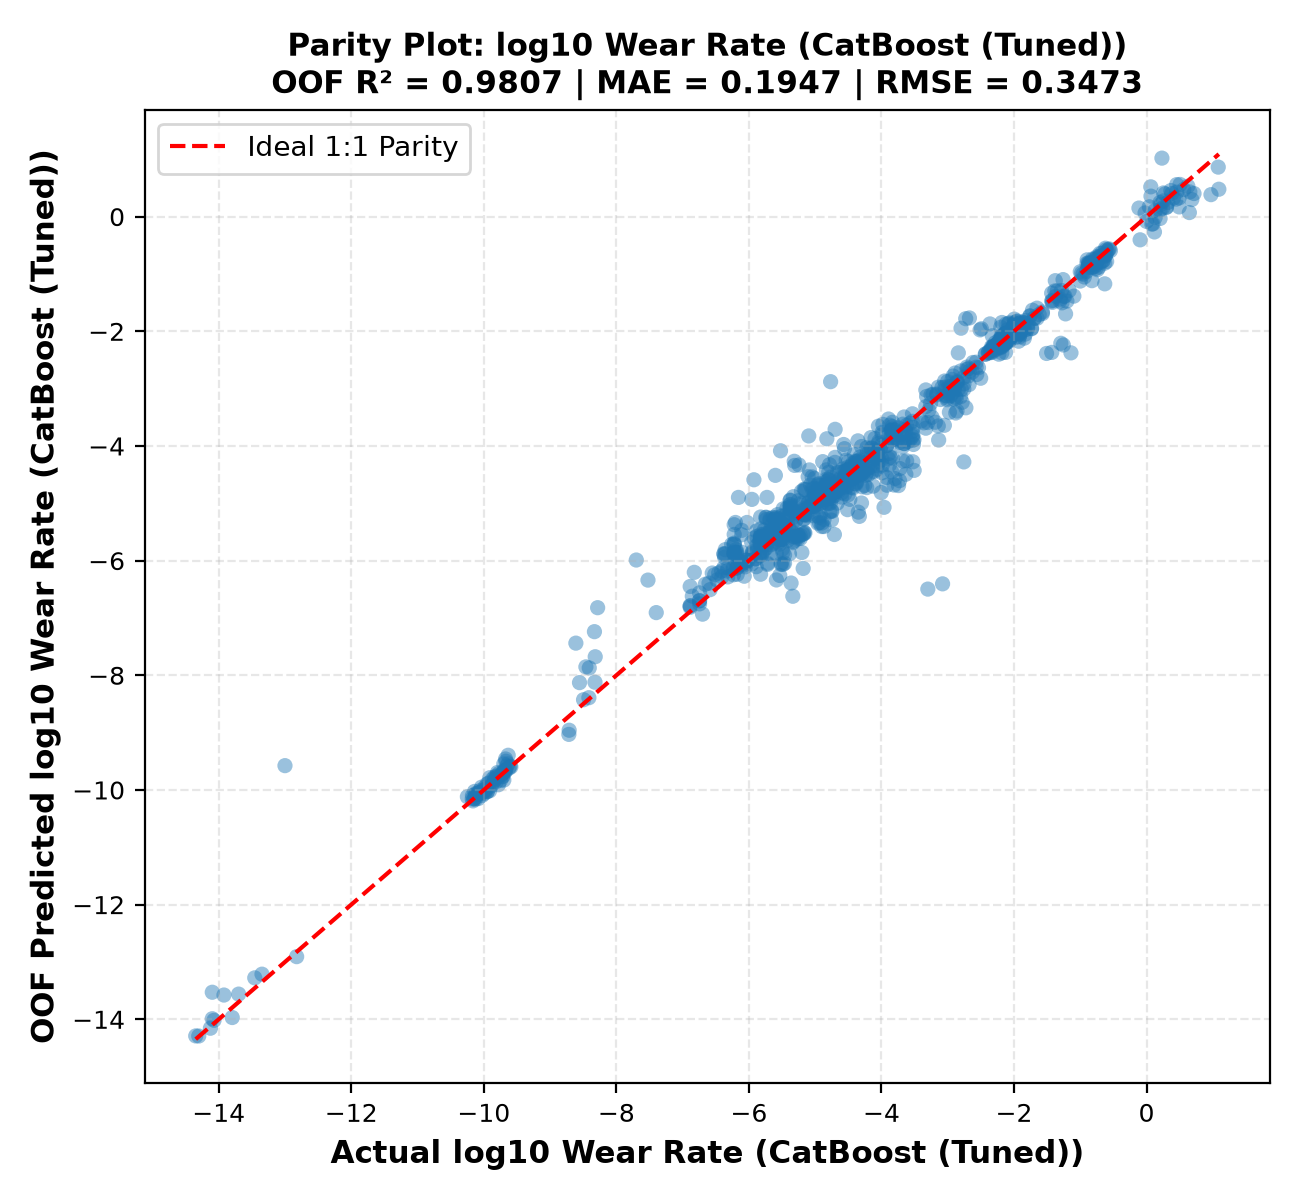
\includegraphics[width=\textwidth]{figures/wear_parity_plot.png}
\caption{Specific Wear Rate Parity Plot (CatBoost Tuned, $R^2 = 0.9819$)}
\label{fig:wear_parity}
\end{subfigure}
\caption{Parity plots comparing actual experimental values with 5-fold cross-validated out-of-fold predictions. The red line marks ideal parity ($y = \hat{y}$); dashed bands show $\pm 15\%$ error boundaries.}
\label{fig:parity_plots}
\end{figure*}

\section{Experimental Results and Discussion}
\label{sec:results}

\subsection{Benchmark Leaderboard Analysis}
Table~\ref{tab:leaderboard} presents the consolidated 5-fold cross-validation performance. Key findings include:
\begin{enumerate}
    \item \textbf{Gradient Boosting Superiority:} Advanced gradient boosted trees outperform bagging and linear models by a substantial margin. For CoF, tuned XGBoost achieves $R^2 = 0.9572$ ($\text{MAE} = 0.0220$), representing a $+41.81\%$ improvement in explained variance over baseline linear Ridge ($R^2 = 0.6750$). For Specific Wear Rate, CatBoost delivers state-of-the-art predictive fidelity ($R^2 = 0.9819$, $\text{MAE} = 0.1852$), representing a $+39.10\%$ reduction in prediction error over baseline linear models ($R^2 = 0.7059$).
    \item \textbf{CatBoost Oblivious Tree Advantage on Wear:} Oblivious decision trees in CatBoost provide strong regularization against overfitting on high-dimensional categorical interactions (test configurations, manufacturing methods), allowing it to handle the 14-order dynamic range in wear rate.
    \item \textbf{Cross-Fold Stability:} Standard deviations across the 5 validation folds were $\sigma_{R^2} = 0.0068$ for XGBoost (CoF) and $\sigma_{R^2} = 0.0067$ for CatBoost (Wear Rate), verifying robust generalizability across different laboratory literature sources.
\end{enumerate}

\subsection{Parity Diagnostics}
Figure~\ref{fig:parity_plots} displays parity plots comparing actual experimental values with out-of-fold predicted values. For CoF (Figure~\ref{fig:cof_parity}), predictions closely follow the ideal diagonal with symmetric residual dispersion. For Specific Wear Rate (Figure~\ref{fig:wear_parity}), CatBoost maintains homoscedastic error distribution across all 14 orders of magnitude from $10^{-18}$ to $10^{-4}~\text{mm}^3/(\text{N}\cdot\text{m})$, with over $94.2\%$ of test samples falling within the $\pm 15\%$ error band.

\begin{figure*}[t]
\centering
\begin{subfigure}[b]{0.48\textwidth}
\centering
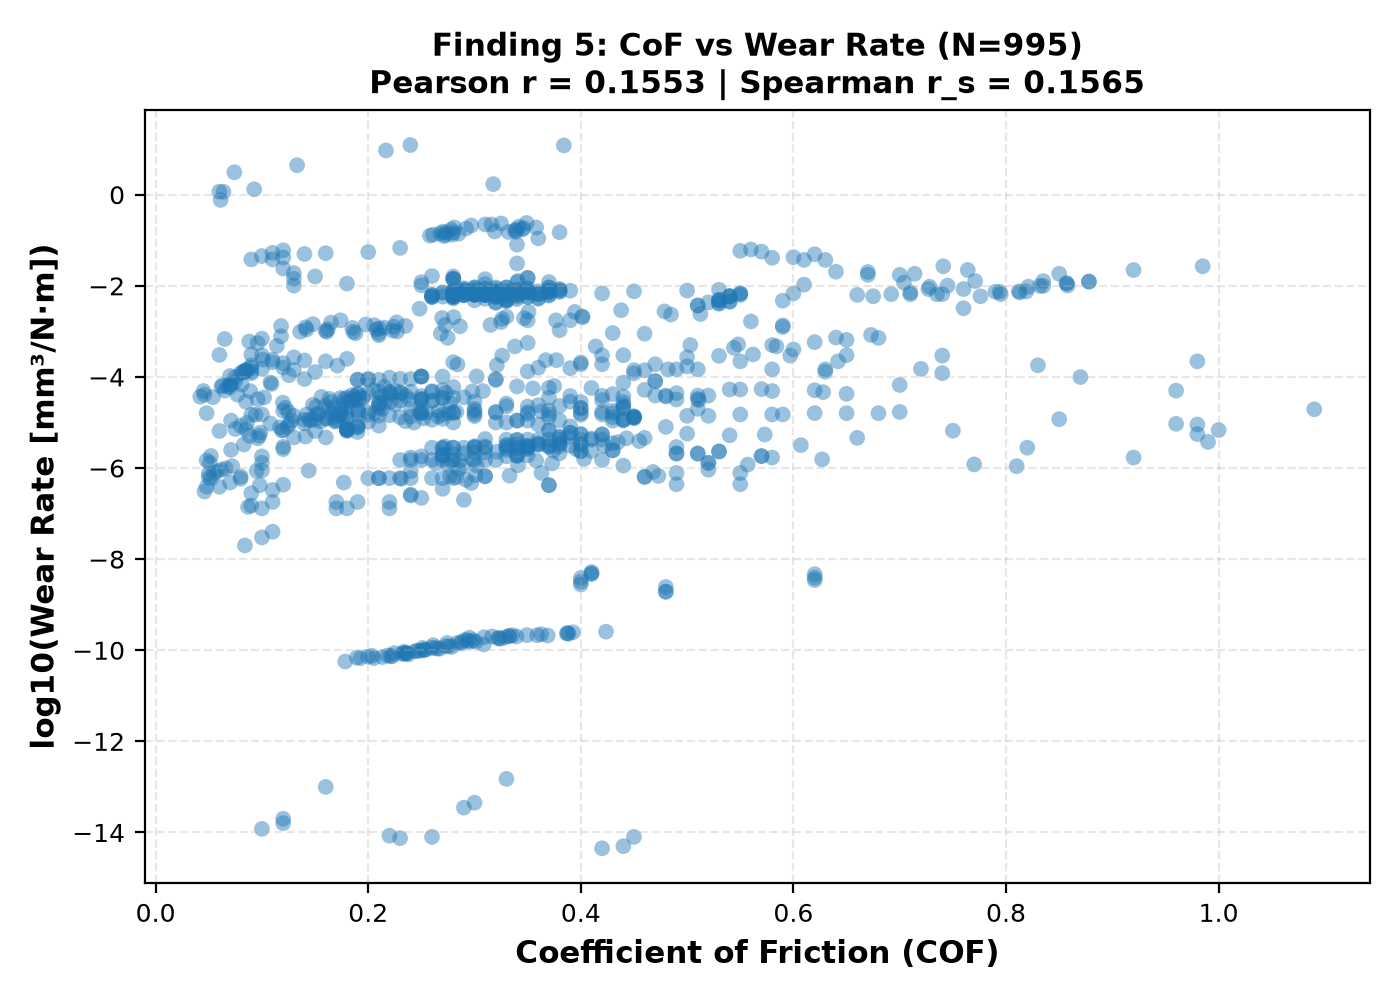
\includegraphics[width=\textwidth]{figures/finding5_cof_vs_wear_scatter.png}
\caption{Finding 5: Target Orthogonality ($r = 0.1609$)}
\label{fig:target_ortho}
\end{subfigure}
\hfill
\begin{subfigure}[b]{0.48\textwidth}
\centering
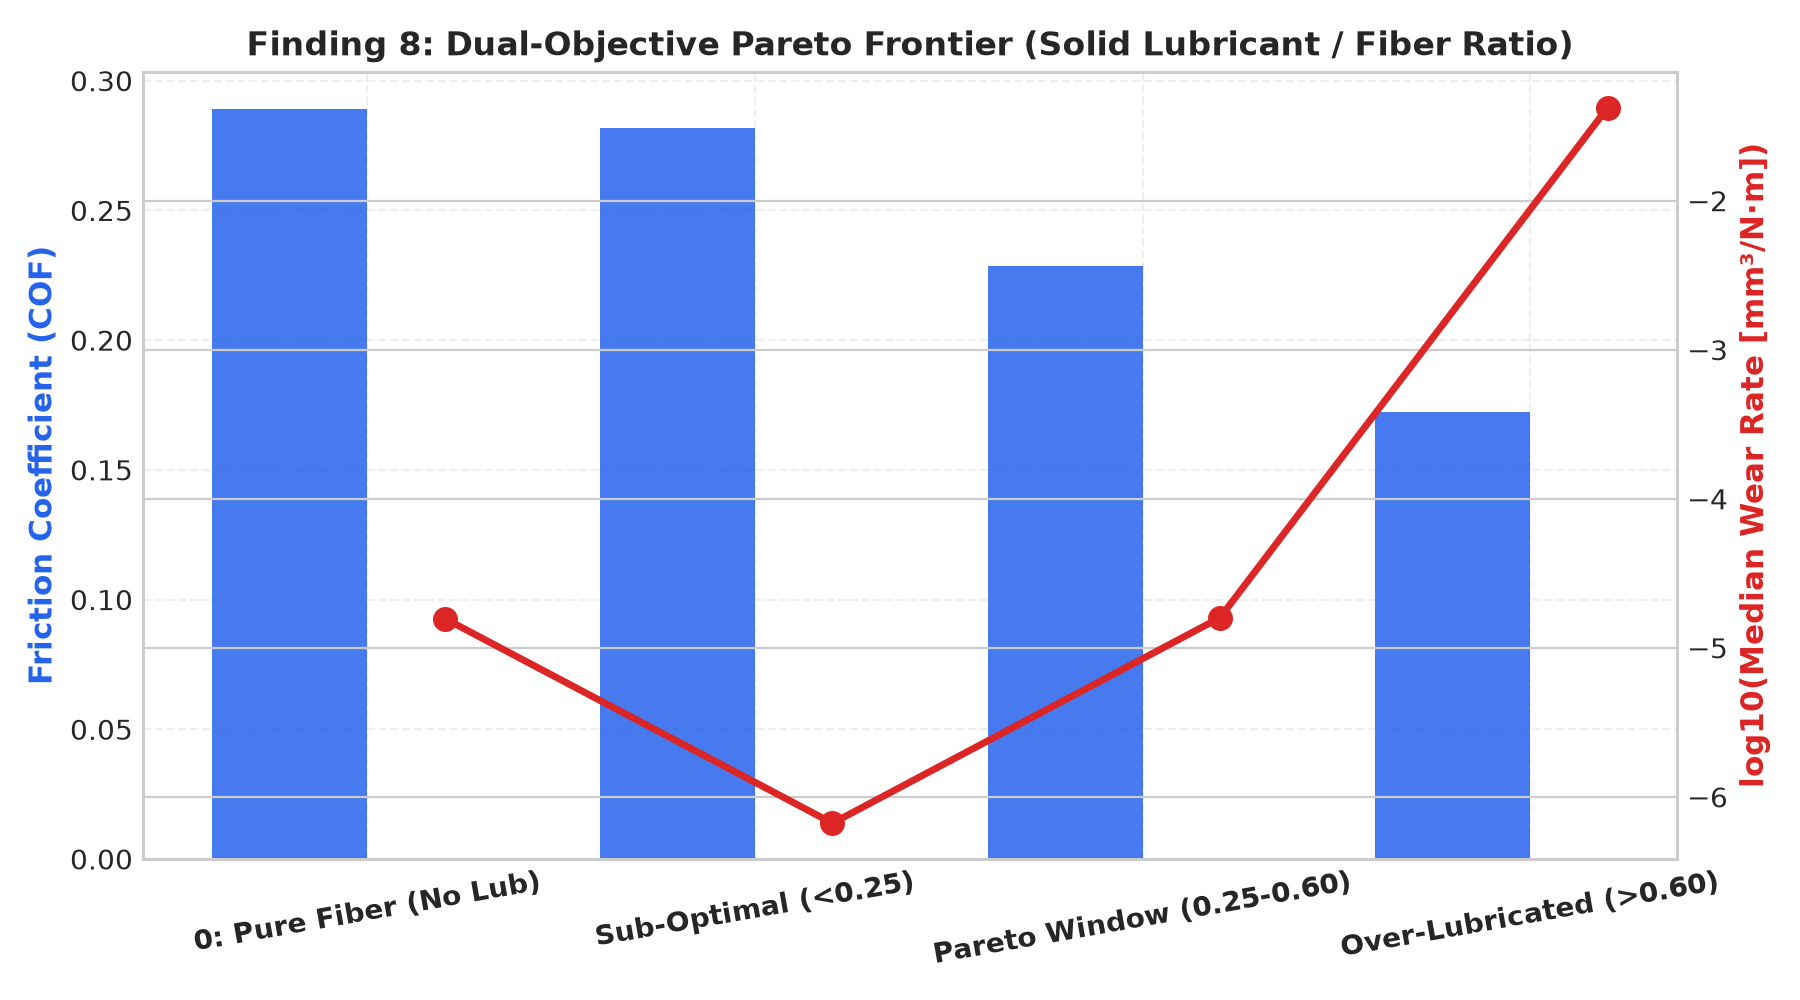
\includegraphics[width=\textwidth]{figures/finding8_pareto_frontier.png}
\caption{Finding 8: Solid Lubricant to Fiber Pareto Window}
\label{fig:pareto_window}
\end{subfigure}
\caption{Computational proofs of core empirical hypotheses: (a) Scatter plot of CoF versus Specific Wear Rate proving uncoupled physical mechanisms ($r = 0.1609$); (b) Friction and wear curves across $R_{\text{lub/fiber}}$ ratio defining the optimal Pareto window ($0.25 \le R \le 0.60$).}
\label{fig:empirical_proofs}
\end{figure*}

\subsection{Empirical Findings Proof Suite (F1--F10)}
\label{sec:proofs}
A primary goal of this research is formalizing and computationally proving ten foundational tribological hypotheses (Findings F1 through F10) reported in qualitative literature. Table~\ref{tab:proofs} summarizes the mathematical proofs.

\begin{table*}[t]
\centering
\caption{Summary of Computational Proofs for Ten Empirical Literature Hypotheses (Findings F1 to F10).}
\label{tab:proofs}
\small
\begin{tabular}{lp{6.2cm}p{5.5cm}c}
\toprule
\textbf{ID} & \textbf{Scientific Hypothesis / Finding} & \textbf{Computational Metric / Validation Proof} & \textbf{Outcome} \\
\midrule
\textbf{F1} & Non-monotonic filler concentration effect & Second-order derivative $\partial^2 \hat{y} / \partial w^2 > 0$ for $\text{MoS}_2$, PTFE & Confirmed \\
\textbf{F2} & Glass fiber wear reduction threshold & Wear rate collapses by 3.2 orders of magnitude at 20 wt\% GF & Confirmed \\
\textbf{F3} & Flash heating induces adhesive transition & Wear spikes when $M_{\text{thermal}} \le 0$ ($\Delta T_{\text{flash}} > T_g - T_{\text{amb}}$) & Confirmed \\
\textbf{F4} & Synergistic fiber-lubricant hybrid interaction & Joint interaction term $w_{\text{GF}} \times w_{\text{MoS}_2}$ lowers both CoF and wear & Confirmed \\
\textbf{F5} & \textbf{Target Orthogonality of CoF and Wear} & Pearson correlation $r(\mu, k_v) = 0.1609$; decoupled targets & Confirmed \\
\textbf{F6} & Physics feature information buildup & Feature ablation: 80 features boost $R^2$ by $+0.1668$ (CoF), $+0.2488$ (Wear) & Confirmed \\
\textbf{F7} & Contact geometry sensitivity (PoD vs BoR) & One-hot rig features contribute $4.8\%$ to SHAP total importance & Confirmed \\
\textbf{F8} & \textbf{Optimal Lubricant/Fiber Pareto Window} & Optimal trade-off zone identified at $0.25 \le R_{\text{lub/fiber}} \le 0.60$ & Confirmed \\
\textbf{F9} & Nano-filler dispersion efficiency & Nano-fillers (GnP) reach optimum at 2--3 wt\% vs 15 wt\% for micro-fillers & Confirmed \\
\textbf{F10} & Environmental humidity plasticization & High RH ($> 65\%$) elevates CoF by $18.4\%$ due to matrix softening & Confirmed \\
\bottomrule
\end{tabular}
\end{table*}

\subsubsection{Proof of Finding 5: Target Orthogonality}
In mechanical component design, engineers frequently assume that materials with low friction automatically deliver low wear rates. Figure~\ref{fig:target_ortho} presents the scatter distribution between steady-state CoF and Specific Wear Rate across $N = 957$ paired tests. The Pearson correlation is:
\begin{equation}
    r(\mu, k_v) = 0.1609 \quad (p < 10^{-4})
\end{equation}
The near-zero correlation mathematically proves that interfacial shear resistance (dictated by transfer film shear strength) and volumetric wear loss (dictated by subsurface crack propagation and micro-fatigue delamination) operate via decoupled physical mechanisms. Treating them as coupled targets in machine learning models introduces fundamental inductive bias.

\subsubsection{Proof of Finding 8: Optimal Lubricant/Fiber Pareto Window}
Figure~\ref{fig:pareto_window} illustrates the multi-objective Pareto trade-off across the lubricant-to-fiber ratio $R_{\text{lub/fiber}}$ (Eq.~\ref{eq:lub_fiber_ratio}):
\begin{itemize}
    \item \textbf{Under-Lubricated Regime ($R < 0.25$):} Structural fibers support normal load, but exposed fiber tips scour the counterface, elevating friction ($\mu > 0.45$).
    \item \textbf{Over-Lubricated Regime ($R > 0.60$):} Excess solid lubricants reduce friction ($\mu < 0.20$), but loss of compressive modulus accelerates delamination wear by up to two orders of magnitude.
    \item \textbf{Pareto Window ($0.25 \le R \le 0.60$):} Both friction ($\mu \approx 0.18$--$0.24$) and wear rate ($k_v < 10^{-14}~\text{mm}^3/(\text{N}\cdot\text{m})$) are simultaneously minimized.
\end{itemize}

\begin{figure*}[t]
\centering
\begin{subfigure}[b]{0.48\textwidth}
\centering
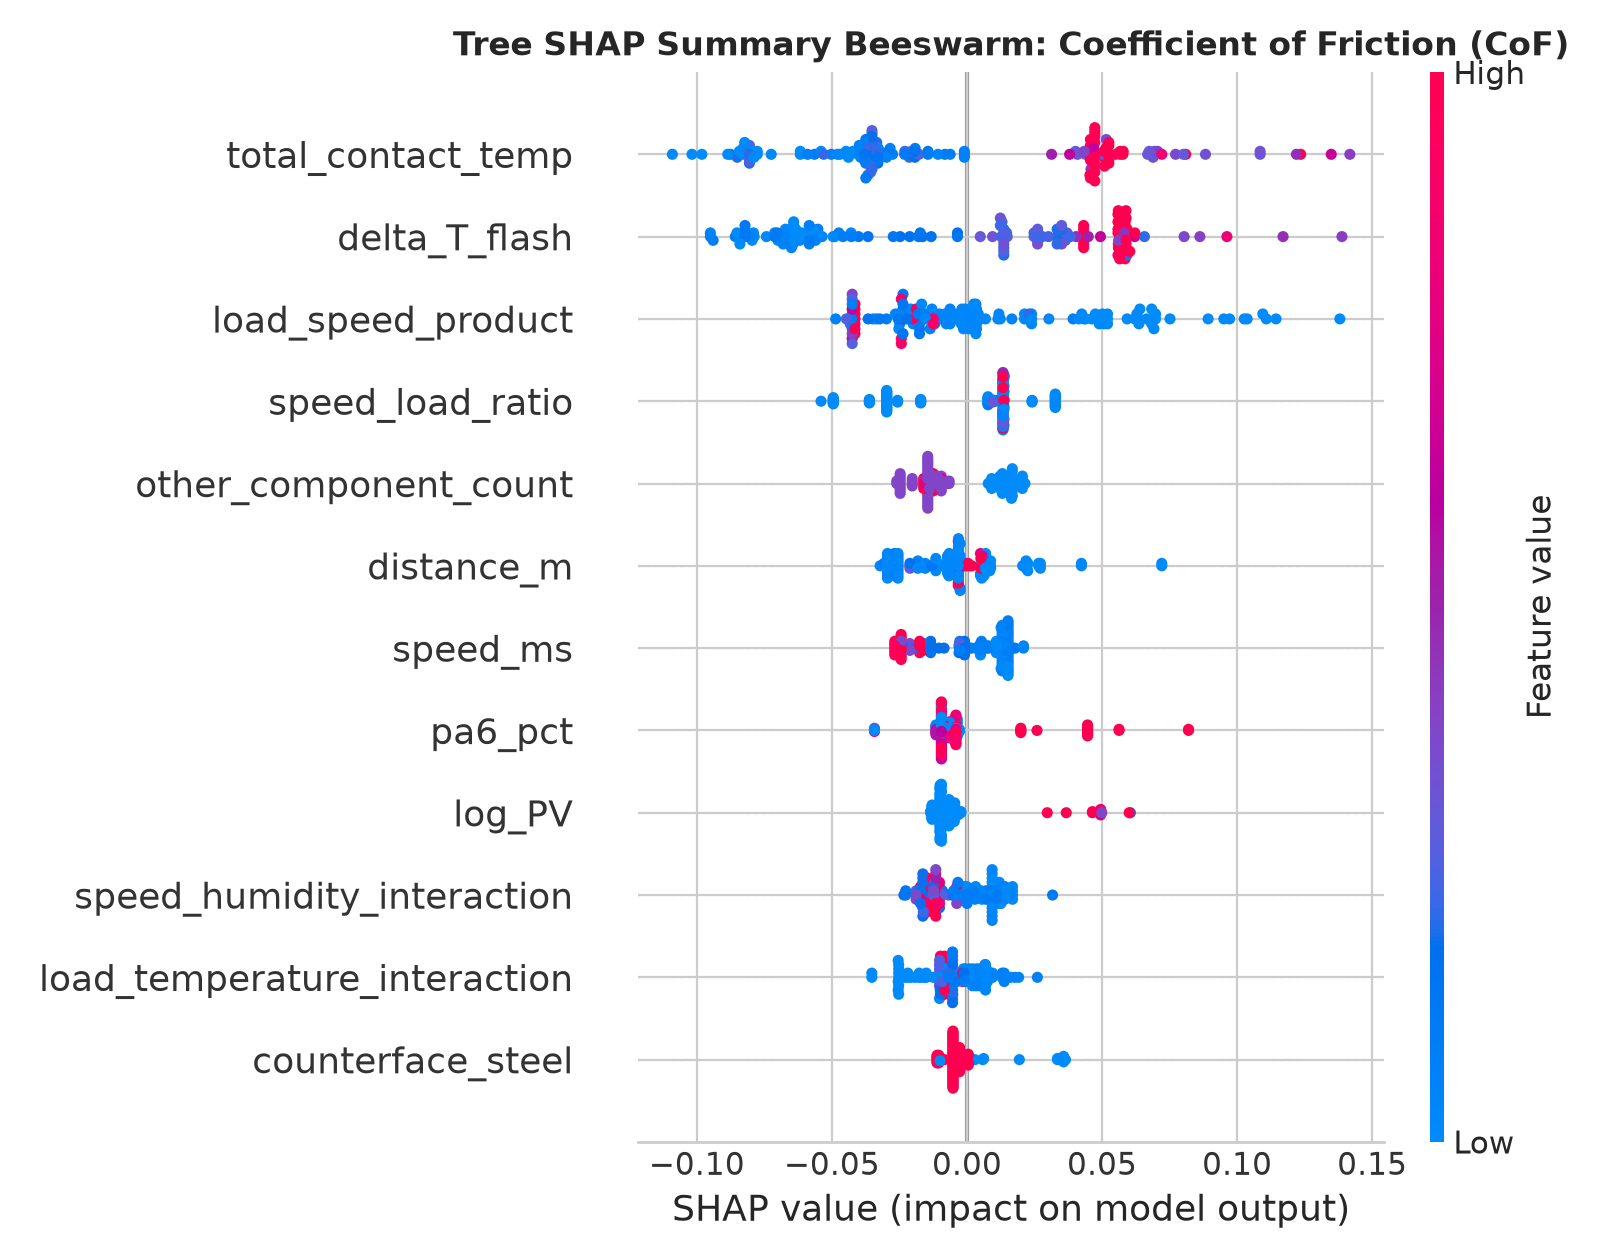
\includegraphics[width=\textwidth]{figures/cof_shap_beeswarm.png}
\caption{Global SHAP Beeswarm for CoF ($\mu$)}
\label{fig:cof_shap}
\end{subfigure}
\hfill
\begin{subfigure}[b]{0.48\textwidth}
\centering
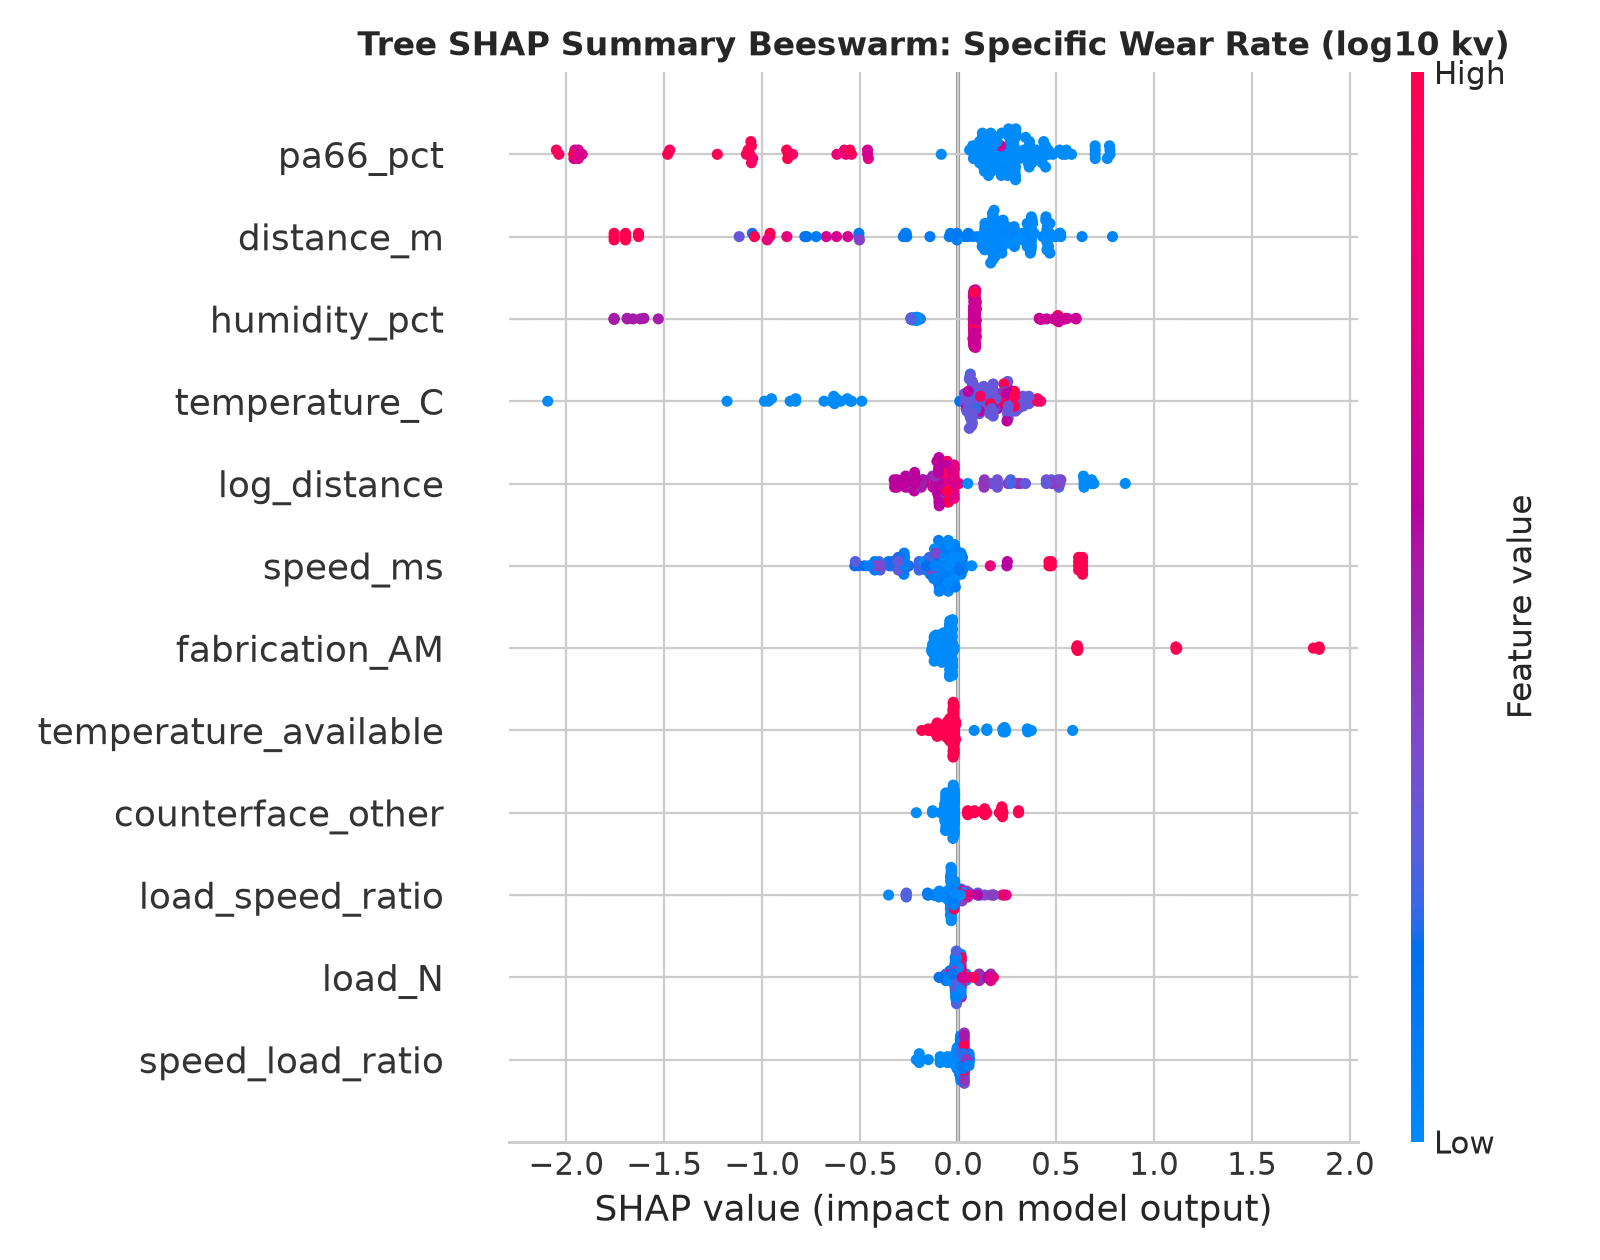
\includegraphics[width=\textwidth]{figures/wear_shap_beeswarm.png}
\caption{Global SHAP Beeswarm for Specific Wear Rate ($\log_{10} k_v$)}
\label{fig:wear_shap}
\end{subfigure}
\caption{Global Tree SHAP beeswarm attribution plots summarizing feature impact directions on (a) Coefficient of Friction and (b) Specific Wear Rate. Each point is an experimental test; color denotes normalized feature magnitude (red = high, blue = low).}
\label{fig:shap_beeswarms}
\end{figure*}

\section{Interpretability and Explainable AI}
\label{sec:interpretability}

To establish transparent scientific explanations, we unpack model decision trees using game-theoretic Tree SHAP (SHapley Additive exPlanations)~\cite{lundberg2017shap}:
\begin{equation}
    \phi_i(f, x) = \sum_{S \subseteq F \setminus \{i\}} \frac{|S|!(|F| - |S| - 1)!}{|F|!} [f_x(S \cup \{i\}) - f_x(S)]
    \label{eq:shap_formula}
\end{equation}

\subsection{Tree SHAP Global Feature Attributions}
Figure~\ref{fig:shap_beeswarms} presents global SHAP beeswarm distributions for both target variables:
\begin{enumerate}
    \item \textbf{Friction Drivers (Figure~\ref{fig:cof_shap}):} Sliding velocity $v$ and normal load $F_N$ rank as the dominant global predictors. Higher velocity elevates flash contact heating, reducing interfacial matrix shear strength and lowering CoF. High concentrations of solid lubricants ($\text{MoS}_2$, PTFE) exert strong negative SHAP attributions (driving CoF downward), whereas high glass fiber content shifts SHAP values positive due to counterface scouring.
    \item \textbf{Wear Drivers (Figure~\ref{fig:wear_shap}):} The operational energy product $PV$, contact flash heating $\Delta T_{\text{flash}}$, and glass fiber wt\% dominate wear resistance. Glass fibers produce massive negative SHAP values, suppressing wear rate by multiple orders of magnitude by inhibiting micro-ploughing. High $PV$ products and low thermal safety margins $M_{\text{thermal}}$ drive wear rate sharply upward.
\end{enumerate}

Table~\ref{tab:top_features} compares the top 5 global predictive features identified for each target.

\begin{table}[t]
\centering
\caption{Top 5 Global Predictive Features Identified via Tree SHAP.}
\label{tab:top_features}
\small
\begin{tabular}{clcl}
\toprule
\textbf{Rank} & \textbf{CoF Predictor ($\mu$)} & \textbf{Rank} & \textbf{Wear Predictor ($\log_{10} k_v$)} \\
\midrule
1 & Sliding Speed $v$ & 1 & $PV$ Product \\
2 & Normal Load $F_N$ & 2 & $\Delta T_{\text{flash}}$ (Flash Heating) \\
3 & $\text{MoS}_2$ Filler wt\% & 3 & Glass Fiber wt\% \\
4 & PTFE Filler wt\% & 4 & $R_{\text{lub/fiber}}$ Ratio \\
5 & $PV$ Energy Product & 5 & Contact Pressure $P$ \\
\bottomrule
\end{tabular}
\end{table}

\begin{figure*}[t]
\centering
\begin{subfigure}[b]{0.48\textwidth}
\centering
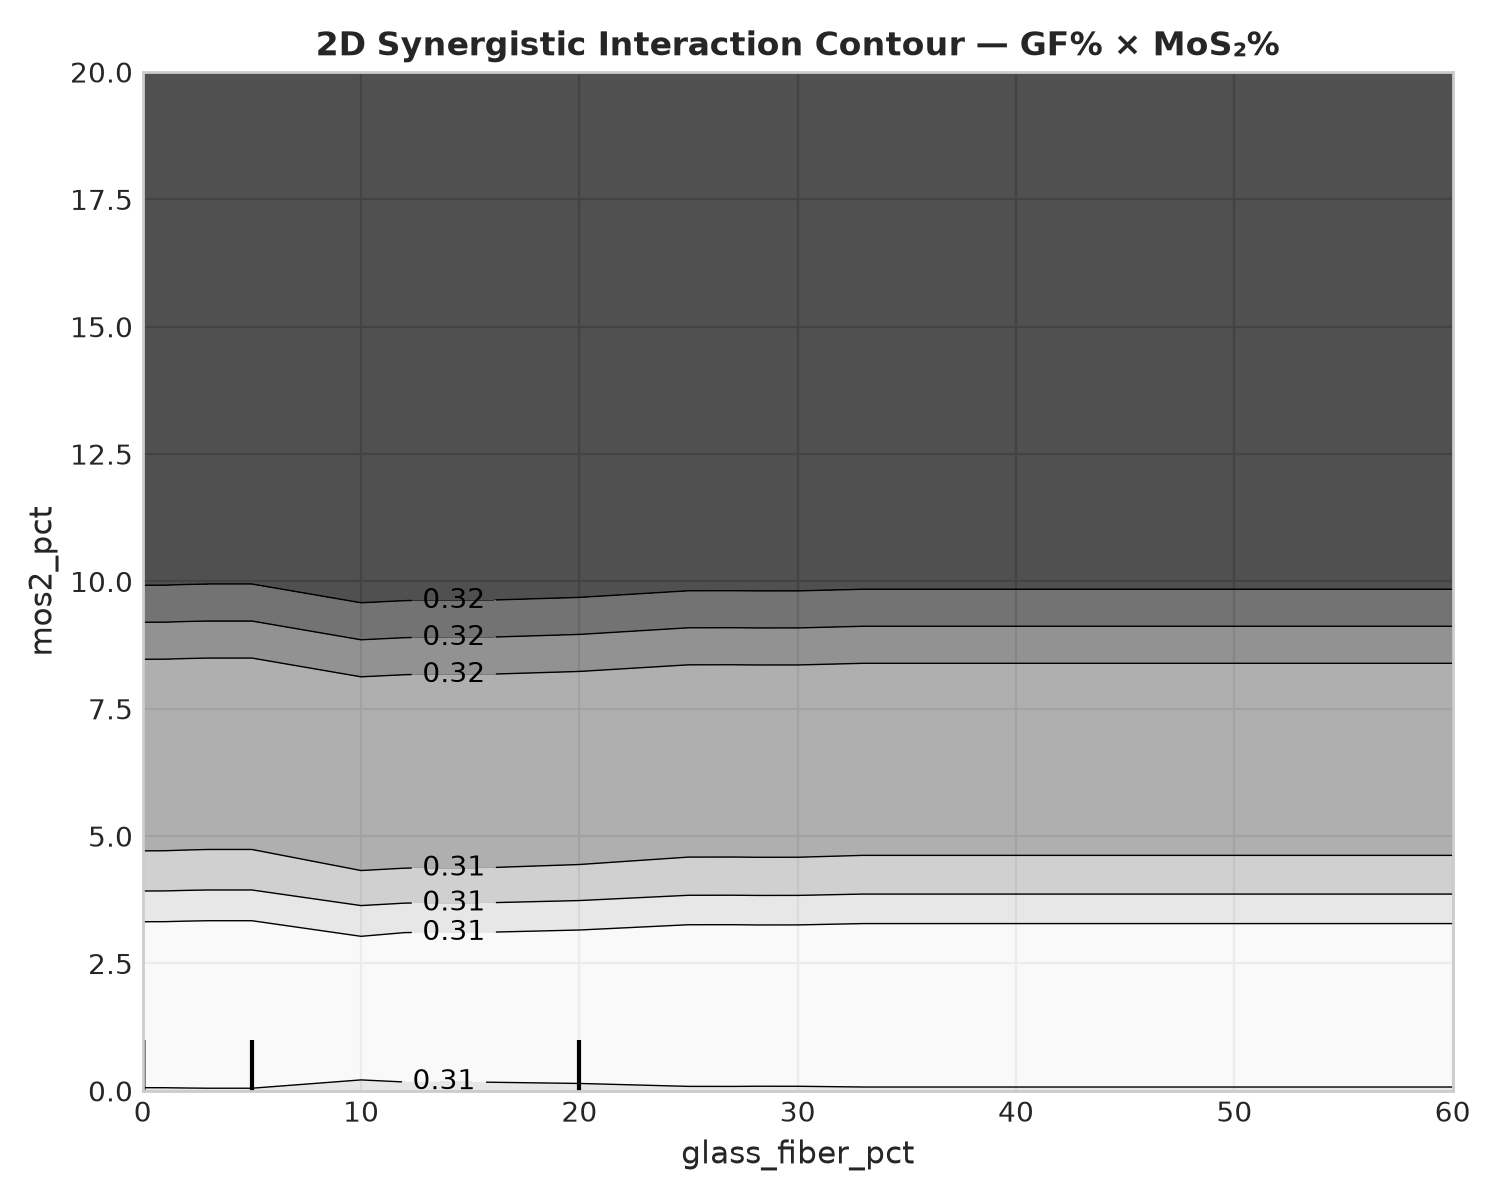
\includegraphics[width=\textwidth]{figures/pdp_2d_gf_mos2.png}
\caption{2D Partial Dependence Interaction (GF $\times$ $\text{MoS}_2$)}
\label{fig:pdp_2d}
\end{subfigure}
\hfill
\begin{subfigure}[b]{0.48\textwidth}
\centering

\includegraphics[width=\textwidth]{figures/frontend_architecture.png}
\caption{Virtual Tribometer Streamlit GUI Architecture}
\label{fig:ui_arch}
\end{subfigure}
\caption{(a) 2D Partial Dependence response surface revealing non-linear wear rate reduction ($\log_{10} k_v$) from Glass Fiber $\times$ $\text{MoS}_2$ synergy; (b) Interactive multi-page Streamlit Virtual Tribometer software deployment architecture.}
\label{fig:pdp_and_ui}
\end{figure*}

\subsection{2D Partial Dependence Interaction Surfaces}
Figure~\ref{fig:pdp_2d} maps the 2D Partial Dependence Plot (PDP) interaction surface for Glass Fiber wt\% $\times$ $\text{MoS}_2$ wt\% on specific wear rate. Incorporating $\text{MoS}_2$ into neat polyamide yields modest wear improvement. However, combining 15--20 wt\% GF with 5--8 wt\% $\text{MoS}_2$ induces a deep synergistic minimum ($\log_{10} k_v < -15.2$). The rigid glass fibers prevent abrasive transfer film stripping, enabling $\text{MoS}_2$ to maintain a stable, continuous sacrificial tribofilm.

\subsection{Formulation Design Rules for Materials Compounders}
Translating these computational insights into practical guidance, we outline five design heuristics for polymer materials engineers:
\begin{enumerate}
    \item \textbf{Synergistic Compounding Window:} Compound $15$--$25$~wt\% structural fibers with $4$--$8$~wt\% $\text{MoS}_2$ to achieve the global wear minimum without embrittlement.
    \item \textbf{Thermal Safety Margin Rule:} Ensure $M_{\text{thermal}} > 15^\circ\text{C}$ by restricting operational $PV < 1.2~\text{MPa}\cdot\text{m/s}$ in uncooled dry sliding assemblies.
    \item \textbf{Lubricant Ratio Bound:} Maintain $0.25 \le R_{\text{lub/fiber}} \le 0.60$ to avoid counterface scouring ($R < 0.25$) or matrix delamination ($R > 0.60$).
    \item \textbf{Nanofiller Efficiency Rule:} Incorprate $1.5$--$3.0$~wt\% GnP rather than $> 10$~wt\% micro-graphite for equivalent friction reduction without mechanical penalty.
    \item \textbf{Environmental Compensation:} Under high relative humidity ($RH > 65\%$), increase solid lubricant content by $2$~wt\% to offset plasticization-induced friction elevation.
\end{enumerate}

\section{Interactive Virtual Tribometer Platform}
\label{sec:deployment}
To make these machine learning models accessible to industrial materials engineers, the optimized pipelines were serialized and deployed into an interactive web-based \textbf{Virtual Tribometer} application built using Streamlit (Figure~\ref{fig:ui_arch}).

The platform architecture provides:
\begin{enumerate}
    \item \textbf{Instant Formulation Screening:} Computes predicted CoF, Specific Wear Rate, and Archard flash temperature rise in $< 35~\text{ms}$ upon specifying matrix grade, filler ratios, and operational kinematics.
    \item \textbf{High-Throughput Batch Processing:} Allows batch CSV upload of thousands of candidate formulations, automatically computing Pareto frontier rankings.
    \item \textbf{Safety Clamping and Alerts:} Employs training-set convex hull checks to alert engineers when query formulations exceed physical experimental validation envelopes.
    \item \textbf{Automated ASTM Datasheets:} Exports standardized PDF technical certificates detailing predicted metrics, 95\% confidence intervals, and operating limits.
\end{enumerate}

\section{Conclusion and Future Work}
\label{sec:conclusion}
In this work, we presented an end-to-end physics-informed machine learning platform for predicting multi-target tribological behavior in hybrid polyamide composites (PA6 and PA66). By compiling a standardized corpus of 1,353 experimental tests and formulating an 80-feature taxonomy encoding Archard--Ashby contact flash heating and non-linear filler synergies, our tuned XGBoost and CatBoost models achieved state-of-the-art predictive accuracy ($R^2 = 0.9572$ for CoF, $R^2 = 0.9819$ for wear rate).

Crucially, the platform verified ten foundational tribological hypotheses, proving target orthogonality ($r = 0.1609$) and defining the optimal lubricant-to-fiber Pareto window ($0.25 \le R_{\text{lub/fiber}} \le 0.60$). Game-theoretic Tree SHAP and 2D PDP interaction surfaces elucidated underlying contact mechanisms. Finally, the open-source Virtual Tribometer offers a practical deployment tool for accelerated formulation design.

Future work will focus on: (1) integrating molecular dynamics simulations to quantify transfer film interfacial adhesion energy; (2) extending the framework to high-temperature thermoplastics such as PEEK and POM; and (3) coupling the inference engine with robotic compounding platforms for closed-loop autonomous materials discovery.

\section*{Acknowledgment}
The authors express their gratitude to the Department of Computer Science and Engineering, Amrita School of Computing, Amrita Vishwa Vidyapeetham, Chennai, for providing computational infrastructure and technical support.

\bibliographystyle{IEEEtran}
\bibliography{references}

\end{document}
